\chapter{Le scelte organizzative}
\thispagestyle{chapterInit}
\section{Costruzione del \texttt{SI}}
    Al momento quando si parla di adottare un nuovo \texttt{SI} si possono fare tre scelte principali:
    \begin{description}
        \item[Make] costruire il \texttt{SI} internamente
        \item[Buy] acquistare il \texttt{SI} da uno o più fornitori esterni
        \item[Outsource] far gestire ad una azienda esterna il \texttt{SI}
    \end{description}
    \subsection{Opzione \textit{make}}
    \label{sec:opzMake}
        Con l'opzione \textbf{make} ovvero di \textbf{costruzione interna} si procede a costruirsi internamente il proprio \texttt{SI} grazie ad un team di sviluppo interno. Questa soluzione prevede però anche l'acquisto e manutenzione della infrastruttura.\newline
        Questa scelta è scelta poche spesso e solitamente si limita a funzioni marginali rispetto ad un \texttt{SI} completo
        \subsubsection{Vantaggi \& Svantaggi} 
        Questa opzione comporta dei costi fissi molto elevati usati sia per il personale che è incaricato di sviluppare e mantenere l'\texttt{SI}, inoltre quando vi è necessità di un aggiornamento importante bisogna investire molte risorse economiche. D'altra parte questa soluzione ha il vantaggio di non confrontarsi con il mercato attuale in quanto è sviluppato sulle esigenze dell'azienda che lo produce e usa. Se si dovessero verificare dei problemi allora i tempi di risoluzione saranno molto brevi per questioni banali ma lunghi per difficoltà più complesse. Altro vantaggio importante di questa soluzione è il mantenimento interno del "\textit{know-how}".
    \subsection{Opzione \textit{buy}}
        \label{sec:opzBuy}
        L'opzione \textbf{buy} consiste nell'acquisto del \texttt{SI} da parte di fornitori esterni. Il gruppo di lavori interno rispetto all'opzione \hyperref[sec:opzMake]{\textit{make}} è molto più ristretto e necessario a gestire l'utenza interna oltre ai rapporti con i fornitori del \texttt{SI}. Questa è una scelta tipica nell'economia italiana delle \texttt{PMI}.
        \subsubsection{Vantaggi \& Svantaggi}
            Come già detto un vantaggio, se non il principale, è quello della ridotta struttura interna, inoltre gli investimenti non sono concentrati su un certo periodo di tempo ma sono smobilizzati. Questo rende l'opzione \textit{buy} maggiormente flessibile rispetto all'opzione \hyperref[sec:opzMake]{\textit{make}} ma ad il costo della stretta dipendenza dalla struttura del fornitore. In questa opzione sicuramente il \textit{know-how} aziendale esce rispetto alla struttura interna, inoltre l'azienda non è proprietaria del software e spesso quest'ultimo è poco personalizzabile. La soluzione è molto aderente col mercato e spesso in confronto con questo.
    \subsection{Opzione \textit{outsource}}
        Con l'opzione di \textbf{outsourcing} ovvero di \textbf{esternalizzazione} si delega ad una terza parte la gestione e l'organizzazione del \texttt{SI} dopo pagamento di canone periodico.
        \subsubsection{hosting}
            Con questa opzione si affida solo la parte di \textbf{infrastruttura} tecnologica, non il software e altri servizi che solitamente vengono gestiti in ottica \hyperref[sec:opzBuy]{\textit{buy}}. Con questa opzione si può noleggiare un server fisico o una macchina virtuale.
        \subsubsection{Body rental}
            Con questo termine intendiamo l'uso di personale specialistico di una azienda esterna per trasformare costi fissi in costi variabili.
        \subsubsection{Vantaggi \& Svantaggi}
            Nell'opzione \textit{outsource} i costi sono variabili ma abbastanza alti, inoltre in caso di necessità si può aumentare o diminuire le risorse in base alle esigenze. Si è però vincolati al fornitore della soluzione utilizzata. È presente inoltre una maggiore flessibilità rispetto all'opzione \textit{make}, come al livello del \textit{buy}. Questa opzione però non permette di avere \textit{know-how} interno e quindi non si ha la possibilità di personalizzare la soluzione in base alle proprie esigenze. Inoltre si ha una maggiore dipendenza dal fornitore del servizio.

\section{Le figure professionali}
    \paragraph{Maturità Informatica} 
        La \textbf{maturità informatica} delle aziende è un indicatore rispetto alla diversa organizzazione e alla collocazione nell'organigramma aziendale del reparto \texttt{IT}, ovvero il reparto che si occupa della gestione del \texttt{SI}. 
    \subsection{Sviluppo del reparto}
        \subsubsection{Livello 1}
            Spesso le aziende a questo livello sono alle fasi iniziali dell'automazione.
            Il team è composto in modo \textbf{orizzontale} senza una organizzazione gerarchica che hanno competenze informatiche simili.
        \subsubsection{Livello 2}
            \begin{figure}[H]
                \centering 
                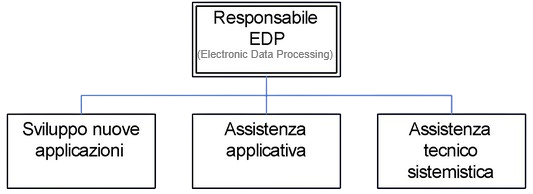
\includegraphics[width=0.5\textwidth]{04/livello2.png}
                \caption{Schema di organizzazione del reparto \texttt{IT} a livello 2}
            \end{figure}
            In questo livello si inizia ad osservare una organizzazione gerarchica dove il \textbf{responsabile \texttt{EDP}} (Electronic Data Processing) è responsabile del reparto \texttt{IT}, sotto di lui ci sono i \textbf{sistemisti} che si occupano della gestione e dell'assistenza sull'infrastruttura. Poi ci sono gli \textbf{analisti} che supportano gli utenti e analizzano i requisiti. Infine ci sono i \textbf{programmatori} che si occupano dello sviluppo del software (non presenti nell'organizzazione \hyperref[sec:opzBuy]{\textit{buy}})
        \subsubsection{Livello 3}
            \begin{figure}[H]
                \centering 
                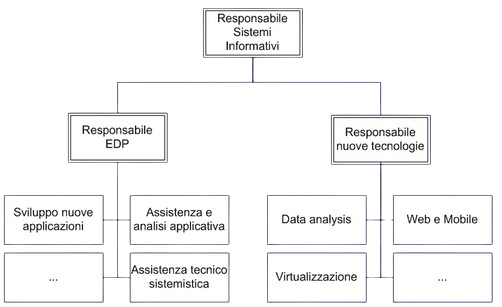
\includegraphics[width=0.5\textwidth]{04/livello3.png}
                \caption{Schema di organizzazione del reparto \texttt{IT} a livello 3}
            \end{figure}
            In questo livello è presente una vera e propria Direzione, sotto questa sono presenti i reparti di \texttt{EDP} e il reparto pero la ricerca su nuove tecnologie. Come mostrato della figura il primo si occupa di sviluppo di nuove applicazioni, assistenza e analisi e assistenza tecnico-sistemistica mentre nel secondo ci si occupa di Analisi dei dati, ricerca web e mobile e virtualizzazione della infrastruttura.
        \subsubsection{Livello 4}
            \begin{figure}[H]
                \centering 
                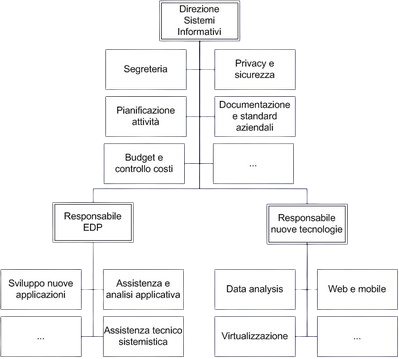
\includegraphics[width=0.5\textwidth]{04/livello4.png}
                \caption{Schema di organizzazione del reparto \texttt{IT} a livello 4}
            \end{figure}
            Livello nel quale è presente un vero e proprio \textbf{dirigente del sistema informativo} con una organizzazione gerarchica molto più complessa rispetto ai livelli precedenti. È presente una divisione \textbf{EDP} con relativo responsabile che è isolata dal reparto \textbf{nuove tecnologie} che si occupa di sviluppare nuove tecnologie e di supportare il reparto \textbf{EDP}. Inoltre sopra di questi è presente una sezione comune del sistema informativo che si occupa di coordinare i due reparti e gestire anche \textbf{privacy} e \textbf{sicurezza} o anche \textbf{pianificazione attività}. Questo livello dispone di un vero e proprio \textbf{budget} per il reparto \texttt{IT}.
    \subsection{Posizione all'interno dell'organigramma}
        \subsubsection{Supporto amministrativo} 
            In questo caso il reparto \texttt{IT} è visto come un supporto amministrativo, questa è una visione obsoleta 
            \begin{figure}[H]
                \centering 
                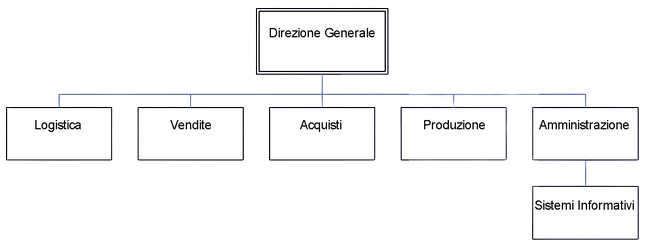
\includegraphics[width=0.5\textwidth]{04/supportoAmm.png}
                \caption{Posizione del reparto \texttt{IT} come supporto amministrativo}
            \end{figure}
        \subsubsection{Servizio ad altre direzioni generali}
            In questo caso il reparto \texttt{SI} è o al pari degli altri reparti o a supporto della direzione generale, in questo caso il reparto \texttt{IT} è messo a supporto degli altri reparti ma è anche uno strumento per la \texttt{DG} per definire processi e strategie, oltre ad avere analisi sui dati.
            \begin{figure}[H]
                \centering 
                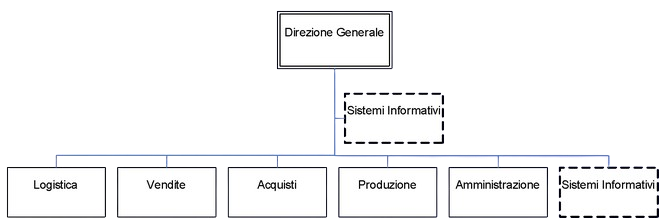
\includegraphics[width=0.5\textwidth]{04/supportoTutti.png}
                \caption{Posizione del reparto \texttt{IT} come supporto a tutte le direzioni}
            \end{figure}
        \subsubsection{Organizzazione autonoma}
            In questo caso è vero che il reparto \texttt{SI} viene messo alle dipendenze del reparto \textbf{organizzazione} ma è anche vero che in questo modello il reparto \texttt{SI} è autonomo. Il suo ruolo è quello di supportare tutte le altre direzioni e di coordinare le varie aree operative dell'azienda, solitamente questo è il modello delle grandi aziende.
            \begin{figure}[H]
                \centering 
                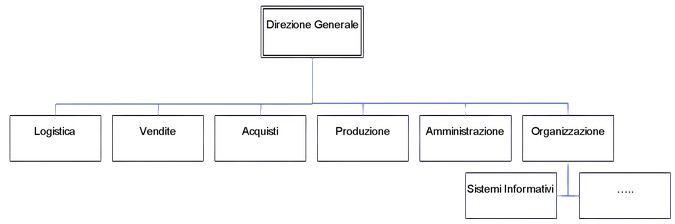
\includegraphics[width=0.5\textwidth]{04/organizzazione.png}
                \caption{Posizione del reparto \texttt{IT} come organizzazione autonoma}
            \end{figure}
\section{Infrastruttura Tecnologica}
    \paragraph{Introduzione} negli anni l'infrastruttura tecnologica si è evoluta siamo passati da server con vari terminali connessi fino alla virtualizzazione a archiviazione in cloud, il tutto passando dall'architettura client-server. Il \texttt{SI} deve tenersi sempre aggiornato con le tecnologie in uso.
    \subsection{Il passaggio da server locali a soluzioni cloud} Recentemente molte aziende stanno eseguendo il passaggio da una infrastruttura locale ad una in cloud, in questo modo sussistono meno investimenti lato \textit{hardware} e \textit{software} che ai giorni nostri invecchiano ancora prima di essere ammortizzati. Tutto il lavoro di gestione dell'infrastruttura è spostato su una azienda esterna senza che venga a mancare l'accessibilità degli strumenti informativi aziendali. In questo modo però si è \textbf{dipendenti dalla connettività} ovvero il lavoro non può essere svolto se non si è connessi a internet.
    \subsection{Interrompibilità del servizio informatico}
        In ogni caso bisogna sempre valutare che danno può causare l'interruzione del servizio informatico. In alcuni casi l'interruzione di esso può portare al blocco totale del lavoro, questo rischio viene spesso sottovalutato dai \textit{top manger}. Come conseguenza è importante garantire la \textit{continuità operativa} ovvero la riduzione o il completo annullamento che un "blocco totale" possa avvenire. 
        \subsubsection{Problematiche legate all'hardware}
            L'infrastruttura dei \texttt{SI} è soggetta a guasti, bisogna dunque prevenire questi andando a implementare il concetto di "\textit{sistema ridondato}\footnote{La ridondanza prevede che in caso di fallimento di un singolo sistema ne esista un'altro che possa sostituirsi ad esso andando a "coprire" il punto difettoso} (esempio per i dischi di archiviazione: \texttt{RAID}).
            \paragraph{\textit{Hot Swap}} Importante per i supporti di archiviazione è anche il concetto di \textit{Hot Swap} che consiste nella possibilità di sostituzione di questi senza dover spegnere il sistema e quindi dover interrompere l'operabilità del \texttt{SI}. 
            \paragraph{\textit{Failure tolerancy}} L'ideale infrastruttura di un \texttt{SI} dovrebbe essere \textit{fault tolerant}, ovvero non deve esistere un oggetto\footnote{server, apparato di rete, griglia elettrica, etc\dots } che in caso di fallimento comporta al fallimento di tutto il sistema, ciò per quelle parti del sistema che sono ritenute essenziali.
            \paragraph{Back-up} Teoria vuole che bisogni avere sempre a disposizione tre copie dei dati su tre apparati diversi: uso, backup interno, backup remoto.
        \subsubsection{Problematiche legate al software}
            Maggiormente le problematiche di un \texttt{SI} sono legate al \textit{software}. I problemi legati a consistono nella "indimostrabilità" che un qualsiasi programma  cerchi di computare un risultato senza "ciclare" all'infinito. D'altra parte questo genere di malfunzionamenti raramente comporta un blocco di tutto il \texttt{SI} ma più spesso interferiscono con un processo specifico o con un gruppo di attività.
        \subsubsection{Problematiche legate ad azioni dolose}
            Molto più frequenti rispetto agli altri generi di criticità sono quelle problematiche legate ad azioni intenti a ledere l'operabilità o la segretezza dei dati. Molto spesso questo genere di problematiche è causato da vulnerabilità dell'\texttt{SI} o dell'\textit{hardware}. La causa principale però rimane l'errore umano che può essere solamente mitigato.\footnote{Più informazioni sulla sicurezza informatica in "Appunti di Introduction to Computer and Network Security" di Luca Facchini, capitoli 1/2}